% Options for packages loaded elsewhere
\PassOptionsToPackage{unicode}{hyperref}
\PassOptionsToPackage{hyphens}{url}
\PassOptionsToPackage{dvipsnames,svgnames,x11names}{xcolor}
%
\documentclass[
  letterpaper,
  DIV=11,
  numbers=noendperiod]{scrartcl}

\usepackage{amsmath,amssymb}
\usepackage{lmodern}
\usepackage{iftex}
\ifPDFTeX
  \usepackage[T1]{fontenc}
  \usepackage[utf8]{inputenc}
  \usepackage{textcomp} % provide euro and other symbols
\else % if luatex or xetex
  \usepackage{unicode-math}
  \defaultfontfeatures{Scale=MatchLowercase}
  \defaultfontfeatures[\rmfamily]{Ligatures=TeX,Scale=1}
\fi
% Use upquote if available, for straight quotes in verbatim environments
\IfFileExists{upquote.sty}{\usepackage{upquote}}{}
\IfFileExists{microtype.sty}{% use microtype if available
  \usepackage[]{microtype}
  \UseMicrotypeSet[protrusion]{basicmath} % disable protrusion for tt fonts
}{}
\makeatletter
\@ifundefined{KOMAClassName}{% if non-KOMA class
  \IfFileExists{parskip.sty}{%
    \usepackage{parskip}
  }{% else
    \setlength{\parindent}{0pt}
    \setlength{\parskip}{6pt plus 2pt minus 1pt}}
}{% if KOMA class
  \KOMAoptions{parskip=half}}
\makeatother
\usepackage{xcolor}
\setlength{\emergencystretch}{3em} % prevent overfull lines
\setcounter{secnumdepth}{-\maxdimen} % remove section numbering
% Make \paragraph and \subparagraph free-standing
\ifx\paragraph\undefined\else
  \let\oldparagraph\paragraph
  \renewcommand{\paragraph}[1]{\oldparagraph{#1}\mbox{}}
\fi
\ifx\subparagraph\undefined\else
  \let\oldsubparagraph\subparagraph
  \renewcommand{\subparagraph}[1]{\oldsubparagraph{#1}\mbox{}}
\fi

\usepackage{color}
\usepackage{fancyvrb}
\newcommand{\VerbBar}{|}
\newcommand{\VERB}{\Verb[commandchars=\\\{\}]}
\DefineVerbatimEnvironment{Highlighting}{Verbatim}{commandchars=\\\{\}}
% Add ',fontsize=\small' for more characters per line
\usepackage{framed}
\definecolor{shadecolor}{RGB}{241,243,245}
\newenvironment{Shaded}{\begin{snugshade}}{\end{snugshade}}
\newcommand{\AlertTok}[1]{\textcolor[rgb]{0.68,0.00,0.00}{#1}}
\newcommand{\AnnotationTok}[1]{\textcolor[rgb]{0.37,0.37,0.37}{#1}}
\newcommand{\AttributeTok}[1]{\textcolor[rgb]{0.40,0.45,0.13}{#1}}
\newcommand{\BaseNTok}[1]{\textcolor[rgb]{0.68,0.00,0.00}{#1}}
\newcommand{\BuiltInTok}[1]{\textcolor[rgb]{0.00,0.23,0.31}{#1}}
\newcommand{\CharTok}[1]{\textcolor[rgb]{0.13,0.47,0.30}{#1}}
\newcommand{\CommentTok}[1]{\textcolor[rgb]{0.37,0.37,0.37}{#1}}
\newcommand{\CommentVarTok}[1]{\textcolor[rgb]{0.37,0.37,0.37}{\textit{#1}}}
\newcommand{\ConstantTok}[1]{\textcolor[rgb]{0.56,0.35,0.01}{#1}}
\newcommand{\ControlFlowTok}[1]{\textcolor[rgb]{0.00,0.23,0.31}{#1}}
\newcommand{\DataTypeTok}[1]{\textcolor[rgb]{0.68,0.00,0.00}{#1}}
\newcommand{\DecValTok}[1]{\textcolor[rgb]{0.68,0.00,0.00}{#1}}
\newcommand{\DocumentationTok}[1]{\textcolor[rgb]{0.37,0.37,0.37}{\textit{#1}}}
\newcommand{\ErrorTok}[1]{\textcolor[rgb]{0.68,0.00,0.00}{#1}}
\newcommand{\ExtensionTok}[1]{\textcolor[rgb]{0.00,0.23,0.31}{#1}}
\newcommand{\FloatTok}[1]{\textcolor[rgb]{0.68,0.00,0.00}{#1}}
\newcommand{\FunctionTok}[1]{\textcolor[rgb]{0.28,0.35,0.67}{#1}}
\newcommand{\ImportTok}[1]{\textcolor[rgb]{0.00,0.46,0.62}{#1}}
\newcommand{\InformationTok}[1]{\textcolor[rgb]{0.37,0.37,0.37}{#1}}
\newcommand{\KeywordTok}[1]{\textcolor[rgb]{0.00,0.23,0.31}{#1}}
\newcommand{\NormalTok}[1]{\textcolor[rgb]{0.00,0.23,0.31}{#1}}
\newcommand{\OperatorTok}[1]{\textcolor[rgb]{0.37,0.37,0.37}{#1}}
\newcommand{\OtherTok}[1]{\textcolor[rgb]{0.00,0.23,0.31}{#1}}
\newcommand{\PreprocessorTok}[1]{\textcolor[rgb]{0.68,0.00,0.00}{#1}}
\newcommand{\RegionMarkerTok}[1]{\textcolor[rgb]{0.00,0.23,0.31}{#1}}
\newcommand{\SpecialCharTok}[1]{\textcolor[rgb]{0.37,0.37,0.37}{#1}}
\newcommand{\SpecialStringTok}[1]{\textcolor[rgb]{0.13,0.47,0.30}{#1}}
\newcommand{\StringTok}[1]{\textcolor[rgb]{0.13,0.47,0.30}{#1}}
\newcommand{\VariableTok}[1]{\textcolor[rgb]{0.07,0.07,0.07}{#1}}
\newcommand{\VerbatimStringTok}[1]{\textcolor[rgb]{0.13,0.47,0.30}{#1}}
\newcommand{\WarningTok}[1]{\textcolor[rgb]{0.37,0.37,0.37}{\textit{#1}}}

\providecommand{\tightlist}{%
  \setlength{\itemsep}{0pt}\setlength{\parskip}{0pt}}\usepackage{longtable,booktabs,array}
\usepackage{calc} % for calculating minipage widths
% Correct order of tables after \paragraph or \subparagraph
\usepackage{etoolbox}
\makeatletter
\patchcmd\longtable{\par}{\if@noskipsec\mbox{}\fi\par}{}{}
\makeatother
% Allow footnotes in longtable head/foot
\IfFileExists{footnotehyper.sty}{\usepackage{footnotehyper}}{\usepackage{footnote}}
\makesavenoteenv{longtable}
\usepackage{graphicx}
\makeatletter
\def\maxwidth{\ifdim\Gin@nat@width>\linewidth\linewidth\else\Gin@nat@width\fi}
\def\maxheight{\ifdim\Gin@nat@height>\textheight\textheight\else\Gin@nat@height\fi}
\makeatother
% Scale images if necessary, so that they will not overflow the page
% margins by default, and it is still possible to overwrite the defaults
% using explicit options in \includegraphics[width, height, ...]{}
\setkeys{Gin}{width=\maxwidth,height=\maxheight,keepaspectratio}
% Set default figure placement to htbp
\makeatletter
\def\fps@figure{htbp}
\makeatother

\KOMAoption{captions}{tableheading}
\makeatletter
\@ifpackageloaded{tcolorbox}{}{\usepackage[many]{tcolorbox}}
\@ifpackageloaded{fontawesome5}{}{\usepackage{fontawesome5}}
\definecolor{quarto-callout-color}{HTML}{909090}
\definecolor{quarto-callout-note-color}{HTML}{0758E5}
\definecolor{quarto-callout-important-color}{HTML}{CC1914}
\definecolor{quarto-callout-warning-color}{HTML}{EB9113}
\definecolor{quarto-callout-tip-color}{HTML}{00A047}
\definecolor{quarto-callout-caution-color}{HTML}{FC5300}
\definecolor{quarto-callout-color-frame}{HTML}{acacac}
\definecolor{quarto-callout-note-color-frame}{HTML}{4582ec}
\definecolor{quarto-callout-important-color-frame}{HTML}{d9534f}
\definecolor{quarto-callout-warning-color-frame}{HTML}{f0ad4e}
\definecolor{quarto-callout-tip-color-frame}{HTML}{02b875}
\definecolor{quarto-callout-caution-color-frame}{HTML}{fd7e14}
\makeatother
\makeatletter
\makeatother
\makeatletter
\makeatother
\makeatletter
\@ifpackageloaded{caption}{}{\usepackage{caption}}
\AtBeginDocument{%
\ifdefined\contentsname
  \renewcommand*\contentsname{Table of contents}
\else
  \newcommand\contentsname{Table of contents}
\fi
\ifdefined\listfigurename
  \renewcommand*\listfigurename{List of Figures}
\else
  \newcommand\listfigurename{List of Figures}
\fi
\ifdefined\listtablename
  \renewcommand*\listtablename{List of Tables}
\else
  \newcommand\listtablename{List of Tables}
\fi
\ifdefined\figurename
  \renewcommand*\figurename{Figure}
\else
  \newcommand\figurename{Figure}
\fi
\ifdefined\tablename
  \renewcommand*\tablename{Table}
\else
  \newcommand\tablename{Table}
\fi
}
\@ifpackageloaded{float}{}{\usepackage{float}}
\floatstyle{ruled}
\@ifundefined{c@chapter}{\newfloat{codelisting}{h}{lop}}{\newfloat{codelisting}{h}{lop}[chapter]}
\floatname{codelisting}{Listing}
\newcommand*\listoflistings{\listof{codelisting}{List of Listings}}
\makeatother
\makeatletter
\@ifpackageloaded{caption}{}{\usepackage{caption}}
\@ifpackageloaded{subcaption}{}{\usepackage{subcaption}}
\makeatother
\makeatletter
\@ifpackageloaded{tcolorbox}{}{\usepackage[many]{tcolorbox}}
\makeatother
\makeatletter
\@ifundefined{shadecolor}{\definecolor{shadecolor}{rgb}{.97, .97, .97}}
\makeatother
\makeatletter
\makeatother
\ifLuaTeX
  \usepackage{selnolig}  % disable illegal ligatures
\fi
\IfFileExists{bookmark.sty}{\usepackage{bookmark}}{\usepackage{hyperref}}
\IfFileExists{xurl.sty}{\usepackage{xurl}}{} % add URL line breaks if available
\urlstyle{same} % disable monospaced font for URLs
\hypersetup{
  pdftitle={Hello R.},
  colorlinks=true,
  linkcolor={blue},
  filecolor={Maroon},
  citecolor={Blue},
  urlcolor={Blue},
  pdfcreator={LaTeX via pandoc}}

\title{Hello R.}
\author{}
\date{}

\begin{document}
\maketitle
\ifdefined\Shaded\renewenvironment{Shaded}{\begin{tcolorbox}[enhanced, boxrule=0pt, breakable, borderline west={3pt}{0pt}{shadecolor}, sharp corners, interior hidden, frame hidden]}{\end{tcolorbox}}\fi

This `lab 0' will introduce you to the course computing workflow. The
main goal of today is to get you setup in RStudio and play around with a
few fundamental skills.

\begin{tcolorbox}[enhanced jigsaw, titlerule=0mm, opacityback=0, breakable, bottomtitle=1mm, bottomrule=.15mm, toptitle=1mm, colbacktitle=quarto-callout-important-color!10!white, left=2mm, arc=.35mm, coltitle=black, toprule=.15mm, colframe=quarto-callout-important-color-frame, opacitybacktitle=0.6, rightrule=.15mm, title=\textcolor{quarto-callout-important-color}{\faExclamation}\hspace{0.5em}{Important}, leftrule=.75mm, colback=white]
This lab will not be graded.
\end{tcolorbox}

\hypertarget{r-and-r-studio}{%
\subsection{R and R Studio}\label{r-and-r-studio}}

Below are the components of the RStudio IDE.

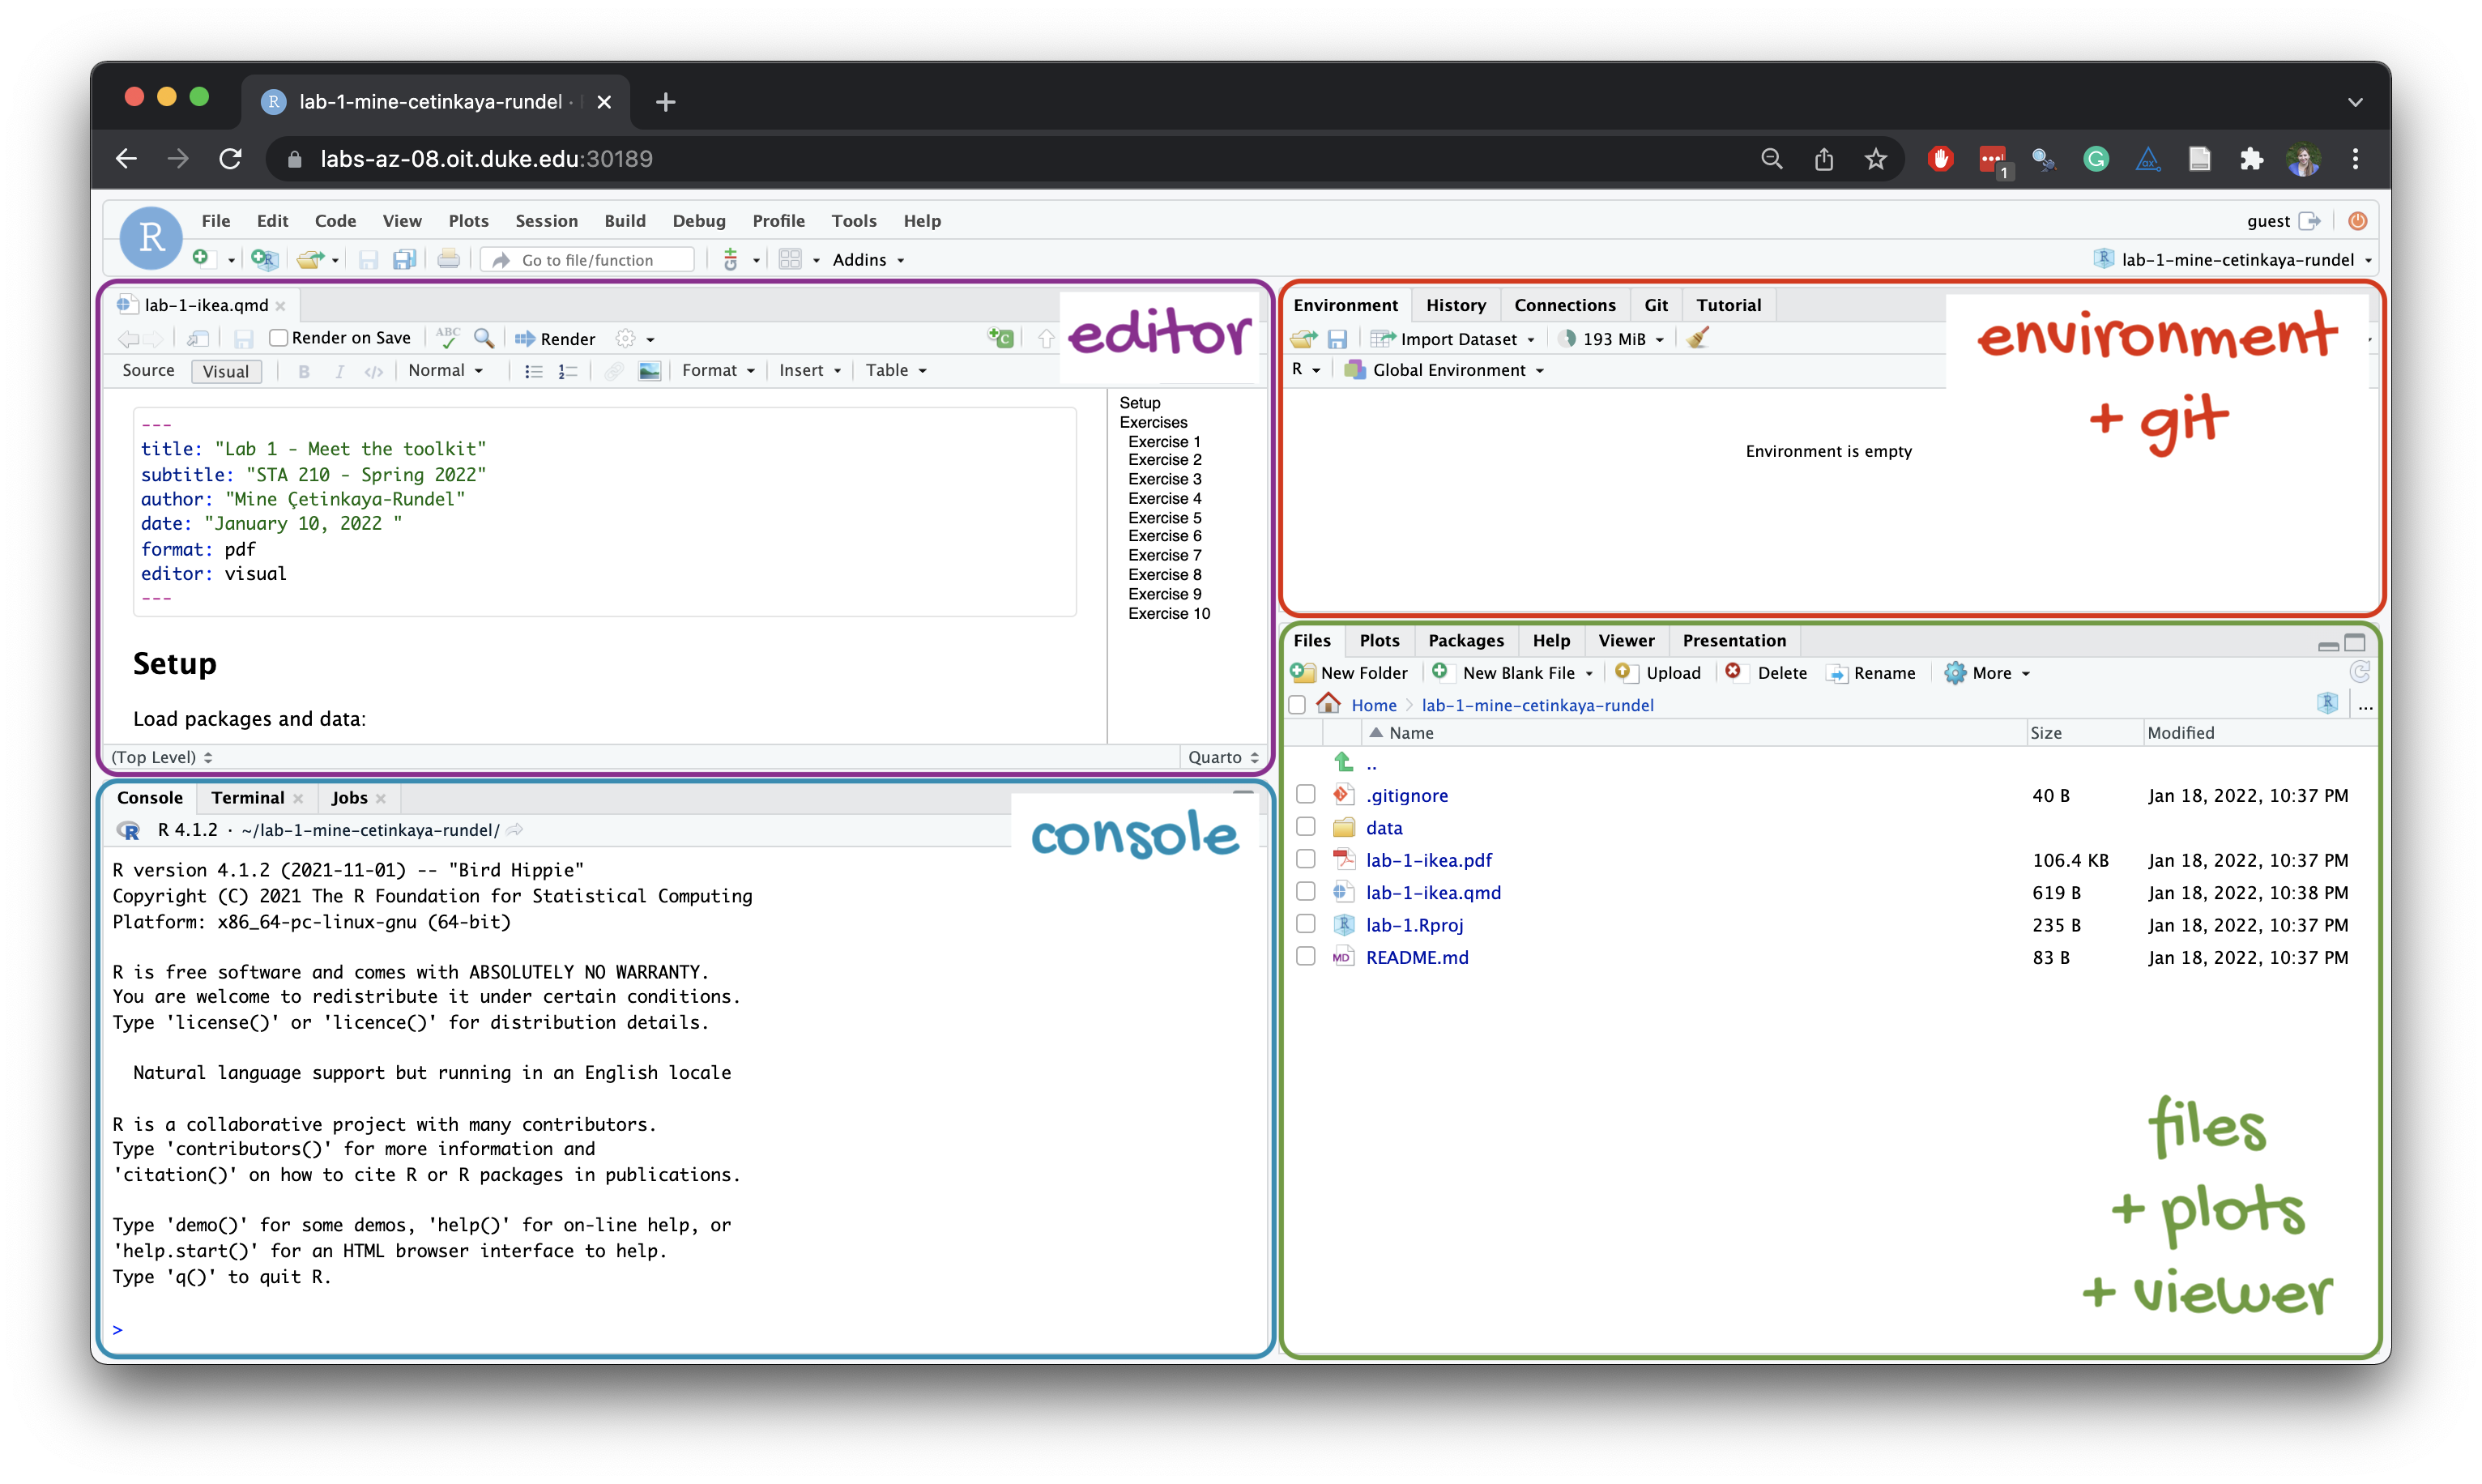
\includegraphics{/slides/images/lab-0/rstudio.png}

Below are the components of a Quarto (.qmd) file. Note: this is
essentially the same as an Rmarkdown (.Rmd) file, with a couple built-in
quality of life additions.

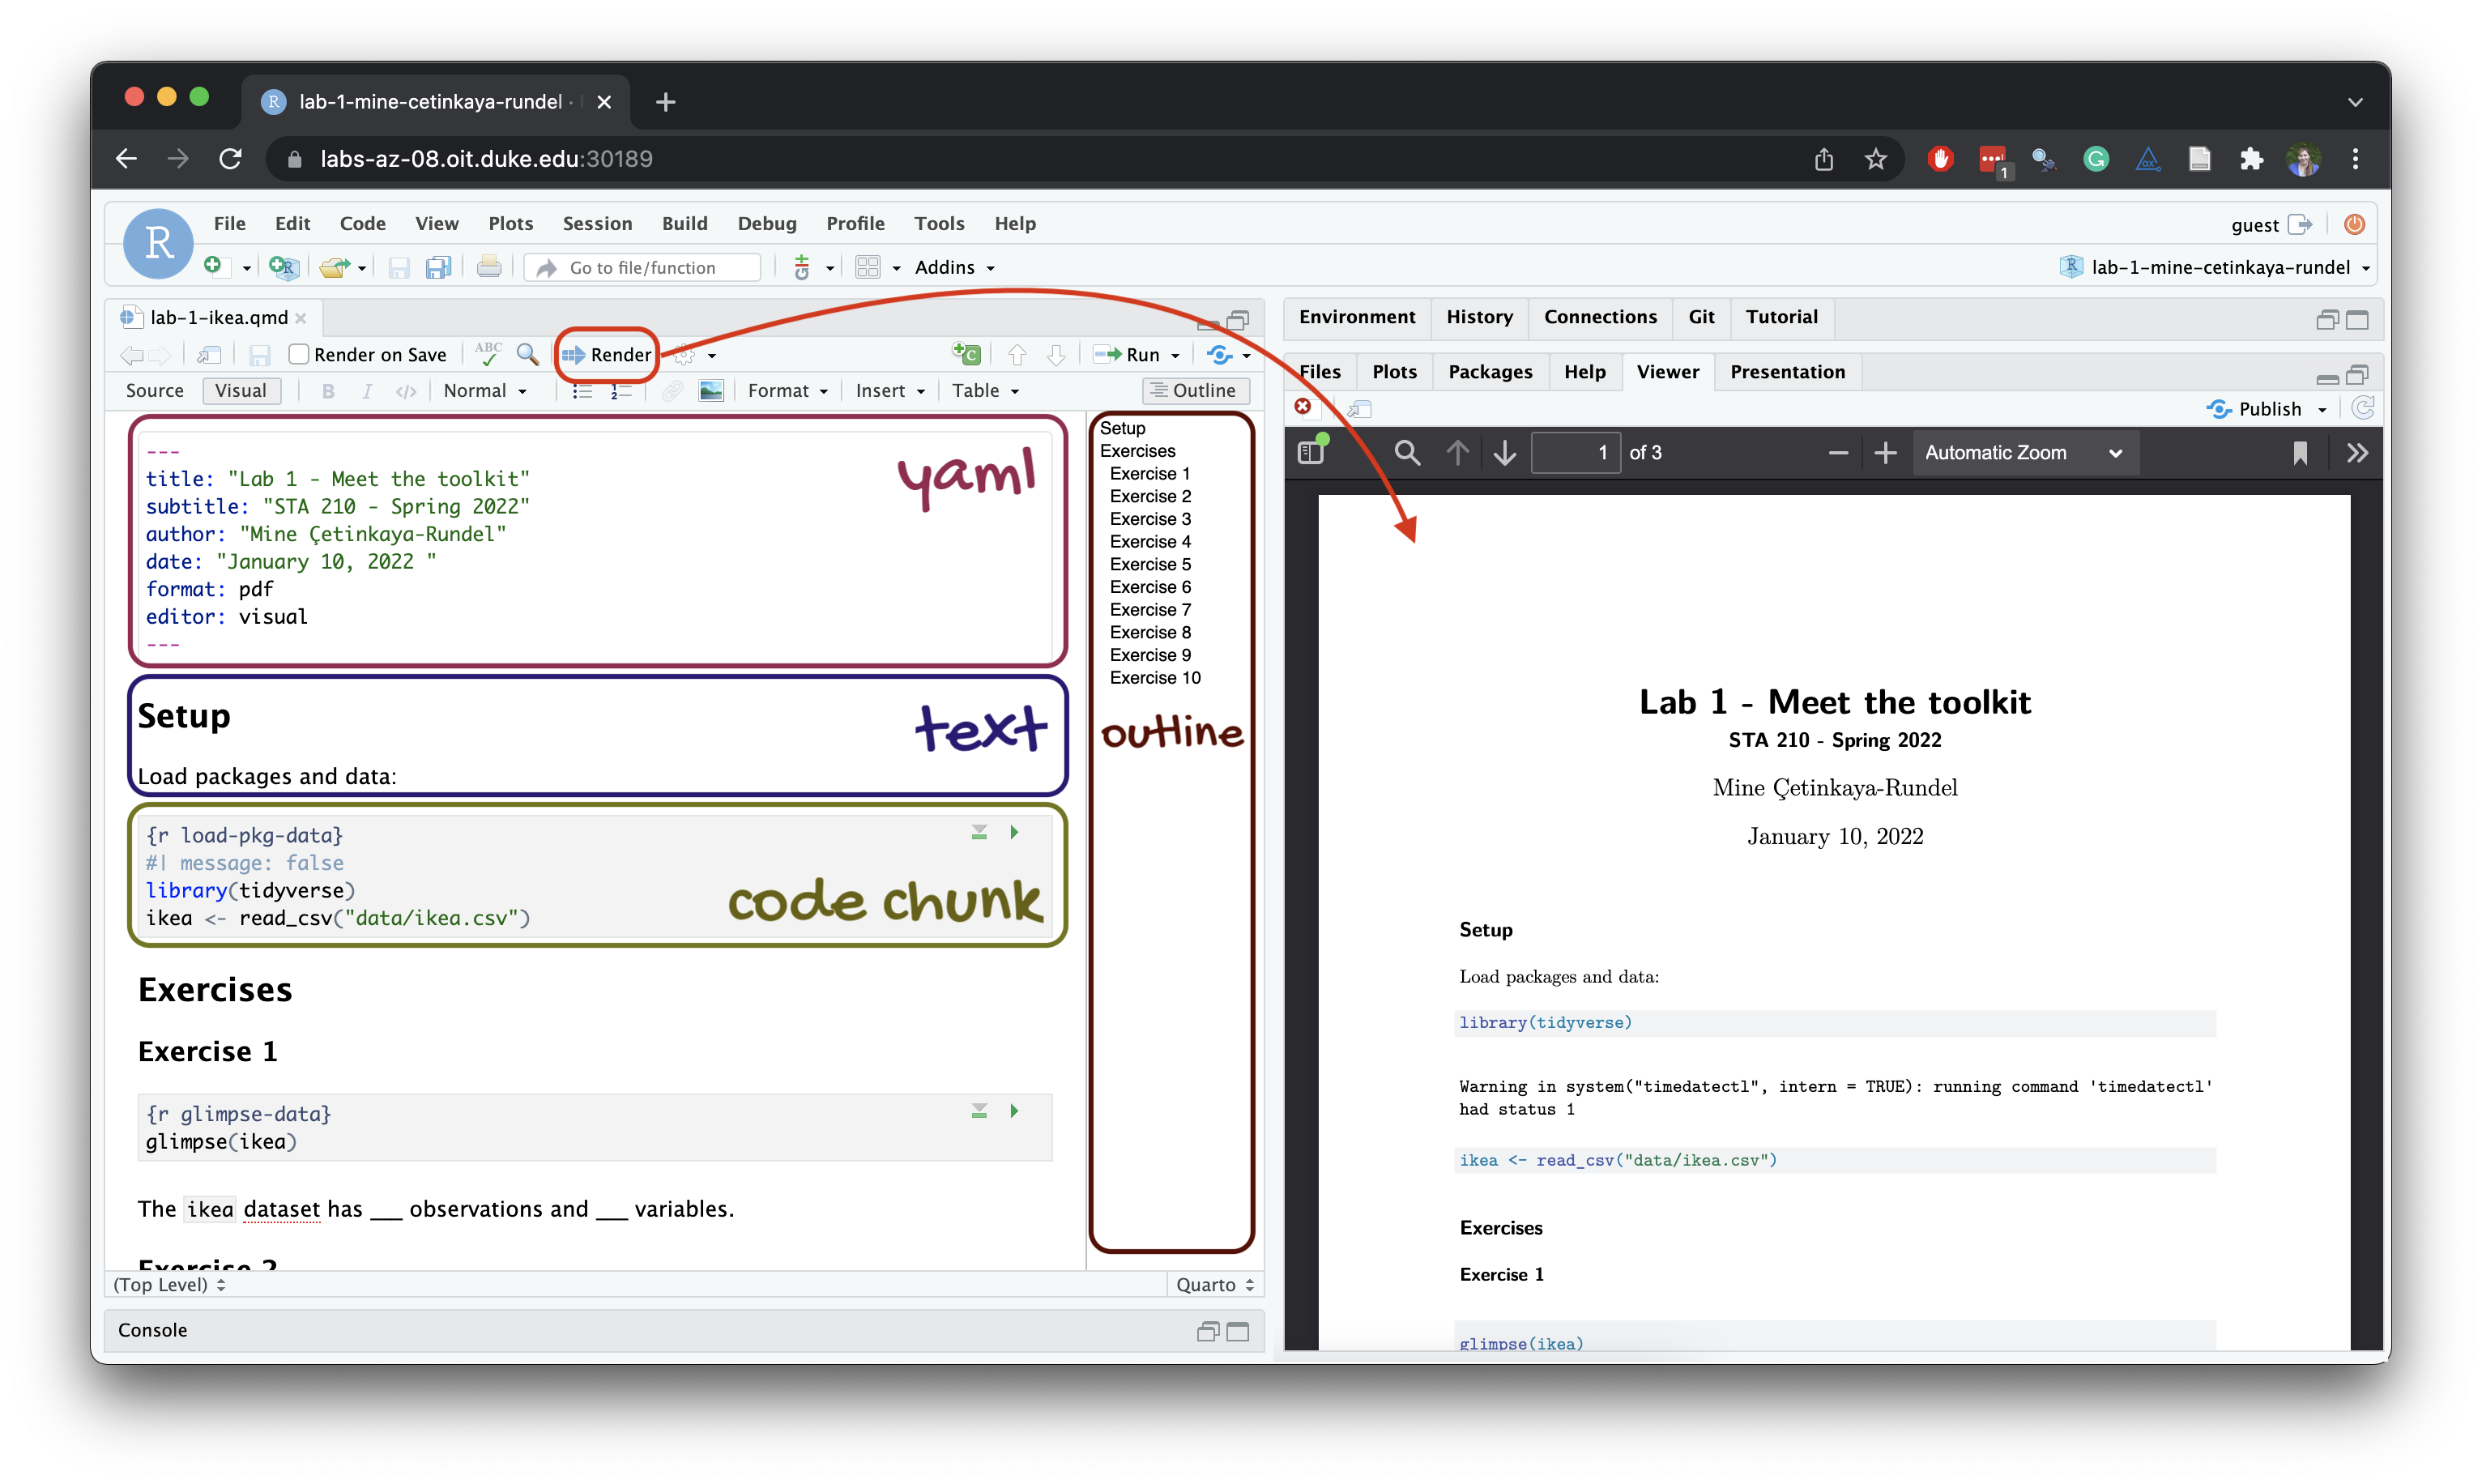
\includegraphics{/slides/images/lab-0/quarto.png}

\hypertarget{yaml}{%
\subsection{YAML}\label{yaml}}

The top portion of your Quarto or R markdown file (between the three
dashed lines) is called \textbf{YAML}. It stands for ``YAML Ain't Markup
Language''. It is a human friendly data serialization standard for all
programming languages. All you need to know is that this area is called
the YAML (we will refer to it as such) and that it contains meta
information about your document.

\begin{tcolorbox}[enhanced jigsaw, titlerule=0mm, opacityback=0, breakable, bottomtitle=1mm, bottomrule=.15mm, toptitle=1mm, colbacktitle=quarto-callout-important-color!10!white, left=2mm, arc=.35mm, coltitle=black, toprule=.15mm, colframe=quarto-callout-important-color-frame, opacitybacktitle=0.6, rightrule=.15mm, title=\textcolor{quarto-callout-important-color}{\faExclamation}\hspace{0.5em}{Important}, leftrule=.75mm, colback=white]
Go to \texttt{file} \textgreater{} \texttt{new\ file},
\texttt{Quarto\ document}. Input title ``Lab 0'', and change the author
name to your name. Select \texttt{pdf} output and press \texttt{Create}.
Render the document. Examine the rendered document.
\end{tcolorbox}

\hypertarget{latex}{%
\subsection{LaTeX}\label{latex}}

Assignments in this course \textbf{are not required} to be written in
LaTeX. You may write equations by hand and scan them as a pdf to submit
to Gradescope. However, LaTeX is \emph{the} typesetting system to
communicate statistics and mathematics professionally. It's worthwhile
to use. Moreover, it's fully supported within .Rmd and .qmd files.

If you're using R on your local machine, you may need to install

\begin{itemize}
\tightlist
\item
  MiKTeX (if you're using windows): \url{https://miktex.org/}
\item
  MacTeX (if you're using macOS): \url{https://www.tug.org/mactex/}
\item
  TeXLive (if you're using linux): \url{https://tug.org/texlive/}
\end{itemize}

To write a LaTeX equation within your markdown document, simply use
\texttt{\$\$} to surround blocks of math and \texttt{\$} to surround
in-line math.

Example: copy and paste the following and then render.

\begin{verbatim}
We can see that $\beta_0 = 2 and \beta_1 = 3$ is the OLS solution under our model

$$
y = \beta_0 + \beta_1 x
$$

\end{verbatim}

\begin{tcolorbox}[enhanced jigsaw, titlerule=0mm, opacityback=0, breakable, bottomtitle=1mm, bottomrule=.15mm, toptitle=1mm, colbacktitle=quarto-callout-note-color!10!white, left=2mm, arc=.35mm, coltitle=black, toprule=.15mm, colframe=quarto-callout-note-color-frame, opacitybacktitle=0.6, rightrule=.15mm, title=\textcolor{quarto-callout-note-color}{\faInfo}\hspace{0.5em}{Note}, leftrule=.75mm, colback=white]
There is no space between \texttt{\$} and math. Whitespace may cause the
document to fail to render.
\end{tcolorbox}

Check out
\href{http://tug.ctan.org/info/undergradmath/undergradmath.pdf}{this
LaTeX cheatsheet} to typeset a variety of math.

\hypertarget{exercises}{%
\subsection{Exercises}\label{exercises}}

The following exercises are designed to help you gain basic familiarity
with R as well as the quirks of floating point arithmetic.

\begin{enumerate}
\def\labelenumi{\arabic{enumi}.}
\tightlist
\item
  Floating point algebra.\\
  \strut \\
  Do floating point numbers obey the rules of algebra? For example, one
  of the rules of algebra is additive association.
  \texttt{(x\ +\ y)\ +\ z\ ==\ x\ +\ (y\ +\ z)}. Check if this is true
  in \texttt{R} using \(x = 0.1\), \(y = 0.1\) and \(z = 1\).
  \textbf{Explain what you find.}
\end{enumerate}

Additional examples of floating point pecularity are provided below.

\begin{Shaded}
\begin{Highlighting}[]
\CommentTok{\# example 1}
\FloatTok{0.2} \SpecialCharTok{==} \FloatTok{0.6} \SpecialCharTok{/} \DecValTok{3}
\CommentTok{\# example 2}
\NormalTok{point3 }\OtherTok{\textless{}{-}} \FunctionTok{c}\NormalTok{(}\FloatTok{0.3}\NormalTok{, }\FloatTok{0.4} \SpecialCharTok{{-}} \FloatTok{0.1}\NormalTok{, }\FloatTok{0.5} \SpecialCharTok{{-}} \FloatTok{0.2}\NormalTok{, }\FloatTok{0.6} \SpecialCharTok{{-}} \FloatTok{0.3}\NormalTok{, }\FloatTok{0.7} \SpecialCharTok{{-}} \FloatTok{0.4}\NormalTok{)}
\NormalTok{point3}
\NormalTok{point3 }\SpecialCharTok{==} \FloatTok{0.3}
\end{Highlighting}
\end{Shaded}

To work around these issues, you could use \texttt{all.equal()} for
checking the equality of two double quantities in R. \textbf{What does
\texttt{all.equal()} do?}

\begin{Shaded}
\begin{Highlighting}[]
\CommentTok{\# example 1, all.equal()}
\FunctionTok{all.equal}\NormalTok{(}\FloatTok{0.2}\NormalTok{, }\FloatTok{0.6} \SpecialCharTok{/} \DecValTok{3}\NormalTok{)}
\CommentTok{\# example 2, all.equal()}
\NormalTok{point3 }\OtherTok{\textless{}{-}} \FunctionTok{c}\NormalTok{(}\FloatTok{0.3}\NormalTok{, }\FloatTok{0.4} \SpecialCharTok{{-}} \FloatTok{0.1}\NormalTok{, }\FloatTok{0.5} \SpecialCharTok{{-}} \FloatTok{0.2}\NormalTok{, }\FloatTok{0.6} \SpecialCharTok{{-}} \FloatTok{0.3}\NormalTok{, }\FloatTok{0.7} \SpecialCharTok{{-}} \FloatTok{0.4}\NormalTok{)}
\NormalTok{point3}
\FunctionTok{all.equal}\NormalTok{(point3, }\FunctionTok{rep}\NormalTok{(.}\DecValTok{3}\NormalTok{, }\FunctionTok{length}\NormalTok{(point3)))}
\end{Highlighting}
\end{Shaded}

\begin{enumerate}
\def\labelenumi{\arabic{enumi}.}
\setcounter{enumi}{1}
\tightlist
\item
  What do these functions do?
\end{enumerate}

Use \texttt{?rnorm} to read the documentation and explain the output of
each of the following:

\begin{Shaded}
\begin{Highlighting}[]
\FunctionTok{rnorm}\NormalTok{(}\DecValTok{10}\NormalTok{, }\AttributeTok{mean =} \DecValTok{1}\NormalTok{, }\AttributeTok{sd =} \DecValTok{2}\NormalTok{)}
\FunctionTok{pnorm}\NormalTok{(}\DecValTok{0}\NormalTok{)}
\FunctionTok{dnorm}\NormalTok{(}\FloatTok{0.5}\NormalTok{)}
\FunctionTok{qnorm}\NormalTok{(}\FloatTok{0.5}\NormalTok{)}
\end{Highlighting}
\end{Shaded}

How is \texttt{dnorm(0.5)} computed? Can you compute it manually?

\begin{enumerate}
\def\labelenumi{\arabic{enumi}.}
\setcounter{enumi}{2}
\tightlist
\item
  Show it numerically
\end{enumerate}

\(X \sim N(\mu, \sigma^2)\) means that \(X\) is normally distributed
with mean \(\mu\) and \textbf{variance} \(\sigma^2\). Show, using
\texttt{rnorm} that if \(X \sim N(0, 1)\) and \(Y \sim N(1, 2)\) that
\(\mathbb{E}(X + Y) = 1\) and \(\mathbb{V}(X + Y) = 3\)

\begin{enumerate}
\def\labelenumi{\arabic{enumi}.}
\setcounter{enumi}{3}
\tightlist
\item
  Control flow
\end{enumerate}

\begin{Shaded}
\begin{Highlighting}[]
\CommentTok{\# for loop example}
\ControlFlowTok{for}\NormalTok{ (i }\ControlFlowTok{in} \DecValTok{1}\SpecialCharTok{:}\DecValTok{5}\NormalTok{) \{}
  \FunctionTok{cat}\NormalTok{(}\StringTok{"Hello"}\NormalTok{, i, }\StringTok{"}\SpecialCharTok{\textbackslash{}n}\StringTok{"}\NormalTok{)}
\NormalTok{\}}

\CommentTok{\# if else example}
\NormalTok{x }\OtherTok{=} \DecValTok{1}
\ControlFlowTok{if}\NormalTok{(x }\SpecialCharTok{\textgreater{}} \DecValTok{0}\NormalTok{) \{}
  \FunctionTok{print}\NormalTok{(}\StringTok{"I\textquotesingle{}m positive x is greater than 0."}\NormalTok{)}
\NormalTok{\} }\ControlFlowTok{else}\NormalTok{ \{}
  \FunctionTok{print}\NormalTok{(}\StringTok{"I\textquotesingle{}m not so positive about x being positive"}\NormalTok{)}
\NormalTok{\}}
\end{Highlighting}
\end{Shaded}

Assume there are 50 days of class. Suppose that, on any given day, there
is a \(X_i\) probability student \(i\) will come to class. Every day you
come to class, you obtain Y points towards your final grade. Every day
that you don't come to class, you obtain Z points towards your final
grade.

Assume \(Y \sim Uniform(1.9, 2)\) and \(Z \sim Uniform(1, 2)\).

Assume student A has a 95\% chance of coming to class any given day (X =
0.95) and student B has a 70\% of coming to class any given day (X =
0.7). While there are more efficient ways to do this, practice using a
\texttt{for} loop, a conditional \texttt{if} statement, \texttt{rbinom}
and \texttt{runif} to simulate one possible final grade for each
student.

\hypertarget{style-guidelines}{%
\subsection{Style guidelines}\label{style-guidelines}}

Although coding is not the primary focus of this course, there are a
short list below of fundamental principles we will follow. Note: some of
these stylistic principles may not be followed in the text!

First, it's easy to write code that runs off the page when you render to
pdf. This happens when you write more than 80 characters in a single
line of code. To ensure this doesn't happen, make sure your code doesn't
have 80 characters in a single line. To enable a vertical line in the
RStudio IDE that helps you visually see the limit, go to \texttt{Tools}
\textgreater{} \texttt{Global\ Options} \textgreater{} \texttt{Code}
\textgreater{} \texttt{Display} \textgreater{} \texttt{Show\ margin}
\textgreater{} \texttt{80}. This will enable a vertical line in your
\texttt{.qmd} files that shows you where the 80 character cutoff is for
code chunks. Instructions may vary slightly for local installs of
RStudio.

\begin{itemize}
\item
  All binary operators should be surrounded by space. For example
  \texttt{x\ +\ y} is appropriate. \texttt{x+y} is not.
\item
  Any and all pipes \texttt{\%\textgreater{}\%} or
  \texttt{\textbar{}\textgreater{}} as well as ggplot layers \texttt{+}
  should be followed by a new line.
\item
  You should be consistent with stylistic choices, e.g.~only use 1 of
  \texttt{=} vs \texttt{\textless{}-} and \texttt{\%\textgreater{}\%} vs
  \texttt{\textbar{}\textgreater{}}
\item
  Your name should be at the top (in the YAML) of each document under
  ``author:''
\end{itemize}

If you have any questions about style, please ask a member of the
teaching team.



\end{document}
